\documentclass[12pt,letterpaper]{article}
\usepackage[spanish, activeacute]{babel} % espanol
\usepackage[latin1]{inputenc} % acentos sin codigo
\usepackage{graphicx} % graficos
\usepackage{multirow} % para las tablas


\usepackage{multirow, array} % para las tablas
\usepackage{float} % para usar [H]



\usepackage[left=2cm,right=2cm,top=2cm,bottom=2cm]{geometry}
\usepackage{graphicx} % figuras
\usepackage{subfigure} % subfiguras

\usepackage{float} % para usar [H]
\usepackage{amsmath}
\usepackage{txfonts}
\usepackage{stackrel} 

\begin{document}
\begin{titlepage}
\begin{center}


\begin{Large}
\textbf{UNIVERSIDAD PRIVADA DE TACNA} \\
\end{Large}


\vspace*{-0.015in}
\begin{figure}[htb]
\begin{center}

\includegraphics[width=5cm]{./imagenes/logo}
\end{center}
\end{figure}
FACULTAD DE INGENIERIA\\
\vspace*{0.05in}
INGENIERIA DE SISTEMAS  \\


\vspace*{0.5in}
\begin{Large}
\textbf{TRABAJO ENCARGADO:} \\
\end{Large}


\vspace*{0.1in}
\begin{large}
Documento Latex\\
\end{large}




\vspace*{0.3in}
\begin{Large}
\textbf{CURSO:} \\
\end{Large}

\vspace*{0.1in}
\begin{large}
BASE DE DATOS II\\
\end{large}

\vspace*{0.3in}
\begin{Large}
\textbf{DOCENTE:} \\
\end{Large}

\vspace*{0.1in}
\begin{large}
Ing.Patrick Cuadros Quiroga\\
\end{large}


\vspace*{0.3in}
\rule{80mm}{0.1mm}\\


\vspace*{0.1in}
\begin{large}
ESTUDIANTE: \\
Lupe Carolina Tapia Ticona\\
\end{large}



\end{center}
\end{titlepage}





\tableofcontents
 \newpage
\listoftables
 \newpage
\listoffigures




\title{TRABAJO ENCARGADO BASE DE DATOS II} 
\author{Lupe carolina Tapia Ticona} 
\maketitle 
\section{Introduccion} 
LaTeX es software libre bajo licencia LPPL..es un sistema de composicion de textos, 
orientado a la creacion de documentos escritos que presenten una alta calidad tipografica. 
Por sus caracteristicas y posibilidades, es usado de forma especialmente intensa en la generacion 
de articulos y libros cientificos que incluyen, entre otros elementos, expresiones matematicas.




\section{Tablas} 
En los libros escolares, las tablas son normalmente utilizadas para recapitular los resultados
 de una investigacion. En general es necesario manejarlas bien para realizar documentos de buena calidad.La gestion de tablas no es muy intuitiva. Las tablas de base son fáciles y presentables, utilizando la misma logica que
  en HTML, pero una tabla un poco mas elaborada requiere de cierto aprendizaje ya que no es muy intuitiva su construccion.
  
\subsection{Tablas}

\begin{table}[htbp]
\begin{center}
\begin{tabular}{|l|l|}
\hline
Pais & Ciudad \\
\hline \hline
Argentina & Buenos Aires \\ \hline
Chile & Santiago \\ \hline
Francia & Paris \\ \hline
Peru & Lima \\ \hline
Bolivia  & La Paz \\ \hline

\end{tabular}
\caption{Tabla muy sencilla.}
\label{tabla:sencilla}
\end{center}
\end{table}



\begin{table}[htb]
\centering
\begin{tabular}{|l|l|l|l|}
\hline
& \multicolumn{3}{c|}{Europa} \\
\cline{2-4}
& Ciudad & Río & Símbolo\\
\hline \hline
\multirow{3}{1cm}{Espana} & Madrid & Manzanares & Cibeles\\ \cline{2-4}
& Sevilla & Guadalquivir & Giralda\\ \cline{2-4}
& Zaragoza & Ebro & Pilar\\ \cline{1-4}
Francia & Paris & Sena & Torre Eiffel\\ \cline{1-4}
\multirow{2}{1cm}{Italia} & Roma & Tiber & San Pedro\\ \cline{2-4}
& Milán & \multicolumn{1}{c|}{-} & Duomo\\ \cline{1-4}
\end{tabular}
\caption{Tabla muy bonita.}
\label{tabla:final}
\end{table}







\begin{table}[htb]
\centering
\begin{tabular}{|l|c|}
\hline
\multicolumn{2}{|c|}{Europa} \\
\hline
País & Ciudad \\
\hline \hline
\multirow{2}{1cm}{Espana} & Madrid \\ \cline{2-2}
& Sevilla \\ \hline
Francia & Paris \\ \hline
\end{tabular}
\caption{Fusionando celdas.}
\label{tabla:fusionandoceldas}
\end{table}



\begin{table}[H]
\centering
\begin{tabular}{p{2cm} p{5cm}}
\hline
Autor & Poema \\
\hline \hline
Espronceda & Con diez canones por banda, viento en popa, a toda vela, no corta el mar, sino vuela un velero bergantin... \\
\hline
Becquer & Volveran las oscuras golondrinas, en tu balcon sus nidos a colgar, y otra vez con el ala, a sus cristales jugando llamaran... \\
\hline
\end{tabular}
\caption{Autores espanoles.}
\label{tabla:autores}
\end{table}




\newpage


\section{Formulas Matematicas}
En la siguiente entrada mostrare algunas instrucciones útiles, cuando estamos escribiendo 
integrales con LaTeX. Nuestro archivo .tex será parecido al siguiente, donde además es importante cargar el paquete {amsmath}:


\subsection{INTEGRALES}

\begin{equation}
y = \int_{x=0}^{x=2 \pi + 10} f(x) \cdot dx
\end{equation}



\begin{equation}
y = \int \limits_{x=0}^{x=2 \pi + 10} f(x) \cdot dx
\end{equation}



\begin{equation}
y = \int \limits_{x=0}^{x=2 \pi + 10} \!\!\!\!\!\!\! f(x) \cdot dx
\end{equation}



\begin{equation}
y = \iint f(x) = \iiint g(x) = \idotsint h(x) 
\end{equation}



\begin{equation}
z = \int _{y=a}^{y=b} \int _{x=g(y)}^{x=h(y)} f(x) \cdot dx \cdot dy
\end{equation} 


\begin{equation}
y = \dfrac{\int_{x=0}^{x=2 \pi + 10} f(x) \cdot dx}{g(x)}
\end{equation}



\begin{equation}
y = \dfrac{\displaystyle \int_{x=0}^{x=2 \pi + 10} f(x) \cdot dx}{g(x)}
\end{equation}




\begin{equation}
\oint_L = \oiint_A = \oiiint_V
\end{equation}

\newpage
\subsection{FRACCIONES}


Ejemplo con fracciones:  $z = \frac{1}{x} + 4$
\begin{equation}
 z = \frac{1}{x} + 4
\end{equation}

Ejemplo con fracciones:  $z = \dfrac{1}{x} + 4$
\begin{equation}
 z = \dfrac{1}{x} + 4
\end{equation}


Ejemplo con fracciones:  $z = \tfrac{1}{x} + 4$
\begin{equation}
 z = \tfrac{1}{x} + 4
\end{equation}



\begin{equation}
 z = \cfrac{1}{2 + \cfrac{1}{\cfrac{z}{1+y}}}
\end{equation}


Ejemplo con fracciones:  $z = \dfrac{1}{x} + 4$
\begin{equation}
 z = \dfrac{1}{x} + 4
\end{equation}




Ejemplo con fracciones:  $z = \dfrac{1}{x} + 4$
\begin{equation}
 z = \dfrac{1}{x} + 4
\end{equation}


\newpage
\subsection{Reacciones Quimicas}


\begin{equation} \label{reac:A2B}
A \rightarrow B
\end{equation}


\begin{equation}
A_{2}^{+} \rightarrow B^{+}
\end{equation}

\begin{equation}
^{1}B \rightleftarrows 2 \cdot C
\end{equation}

\begin{equation}
C \xrightarrow[a]{b} D
\end{equation}

\begin{equation} 
D \rightarrow E\uparrow + F\downarrow
\end{equation}


\begin{equation}
\mathrm{NO_{3}^{-} + S_{2}O_{7}^{2-} \xrightarrow[T\uparrow]{H^{+}} NO_{2}^{+} + 2 SO_{4}^{2-}}
\end{equation}


\begin{equation}
A + B \stackbin[T_1]{P_1}{=} C + D
\end{equation} 
\newpage
\subsection{Matrcices}


\begin{equation}
\begin{array}{cc}
a & b \\
ccc & d
\end{array}
\end{equation}


\begin{equation}
\left(
\begin{array}{cccc}
1 & 0 & \cdots & 0 \\
0 & 1 & \cdots & 0 \\
\vdots & \vdots & \ddots & \vdots \\
0 & 0 & \cdots & 1
\end{array}
\right)
\end{equation}




\begin{equation}
f(x) = \left\lbrace
\begin{array}{ll}
\textup{si } x>5 & 1\\
\textup{si } x\leq 5 & 0
\end{array}
\right.
\end{equation}





\begin{equation}
\begin{array}{llllll}
& x_1 &&& = & 10 \\
+ \\
& x_1 & + & x_2 & = & 1\\
\cline{2-6}
& 2x_1 & + & x_2 & = & 11
\end{array}
\end{equation}


\begin{eqnarray}
\nonumber x = 1 + 2 + 3 + \\
+ 4 + 5
\end{eqnarray}





\newpage

\section{Graficos} 
\subsection{peliculas Destacadas}

\begin{figure}[htb]
\centering

\includegraphics[width=0.5\textwidth]{./imagenes/1}
\caption{Malefica.} \label{ima:1}
\end{figure}



\begin{figure}[htbp]
\centering
\subfigure[1]{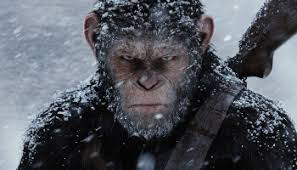
\includegraphics[width=40mm]{./imagenes/9}}
\subfigure[2]{
\includegraphics[width=40mm]{./imagenes/7}}
\subfigure[3]{
\includegraphics[width=80mm]{./imagenes/8}}
\caption{Kit de la pelicula de los simios.} \label{ima:5}
\end{figure}

\newpage
\begin{figure}[htb]
\centering
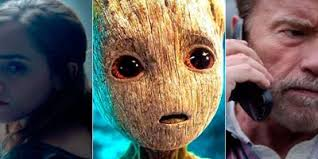
\includegraphics[width=0.5\textwidth]{./imagenes/6}
\caption{Guardianes de la galaxia.} \label{ima:6}
\end{figure}


\begin{figure}[htb]
\centering

\includegraphics[width=0.5\textwidth]{./imagenes/4}
\caption{Alicia en pais de la maravilla.} \label{ima:4}
\end{figure}




\newpage




\section{Bibliografia} 
@ARTICLE{Alfonso2010a,
author = {M. Alfonso and B. Bernardo and C. Carlos and D. Domingo},
title = {El problema de los gatos y los perros},
journal = {Mascotas},
year = {2010},
volume = {50},
pages = {112-115}
}

@ARTICLE{Alfonso2010b,
author = {M. Alfonso and M. Marta and N. Nuria},
title = {Mi viaje a {EEUU}},
journal = {Revista de viajes},
year = {2010},
volume = {14},
pages = {50-56}
}

@ARTICLE{Patricio2011,
author = {A. Patricio},
title = {Una estrella rosa en el fondo del mar},
journal = {El mar},
year = {2011},
volume = {3},
pages = {1071-1090}
}

@ARTICLE{Zacarias2009,
author = {R. Zacarias and G. Graciela},
title = {¿{C}uál te gusta más?},
journal = {Flores},
year = {2009},
volume = {5},
pages = {45-49}
}


















\end{document}